\chapter{Lecture 28 - Departure from Nucleate Boiling in a PWR Core}
\label{ch:ch28}
\section{Objectives}
The objectives of this lecture are:
\begin{enumerate}
\item Qualitatively review DNB as a mechanism for CHF in a PWR core.
\item List some important correlations used to predict DNB.
\item Demonstrate the use of the Tong 68 correlation for DNB and illustrate variation with important parameters.
\end{enumerate}

\section{Departure from Nucleate Boiling}

\begin{marginfigure}
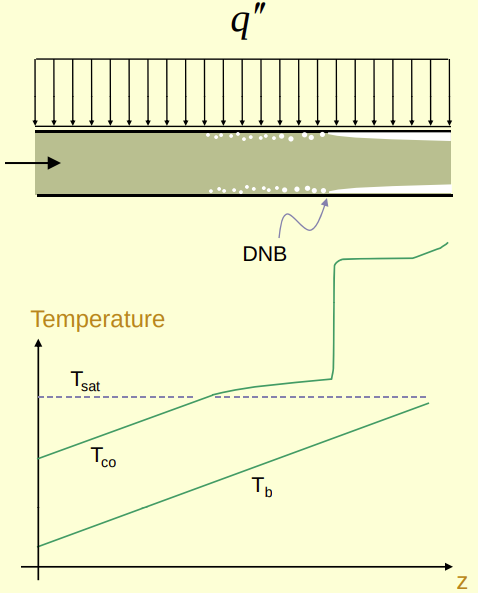
\includegraphics{simple-channel-dnb-schematic.png}
\caption{Simplified channel schematic illustrating departure from nucleate boiling.}
\label{fig:simple-channel-dnb-schematic}
\end{marginfigure}
\newthought{Consider again} the simplified channel with constant heat flux along the wall, this time, as pictured in Figure \ref{fig:simple-channel-dnb-schematic}.
\begin{itemize}
\item Sub-cooled liquid enters the channel but as bulk and wall temperature increases, and wall temperature exceeds saturation temperature for the coolant, nucleate boiling begins.
\item The vapor bubbles formed during nucleate boiling are swept away from the wall and collapse within the sub-cooled bulk coolant but, since coolant equilibrium quality continues to increase, the rate of bubble formation continues to increase.
\item If heat flux is high enough and bulk fluid conditions permit, it may become the case that bubbles are formed at nucleation sites more rapidly than they are swept away in the coolant.
\item Ultimately the wall becomes coated with a layer of vapor bubbles which impedes heat transfer; wall temperature increases rapidly which further contributes to vapor bubble formation along the wall and further degradation of convective heat transfer.
\item This last state is referred to as \emph{departure from nucleate boiling}, or DNB.
\end{itemize}
\begin{marginfigure}
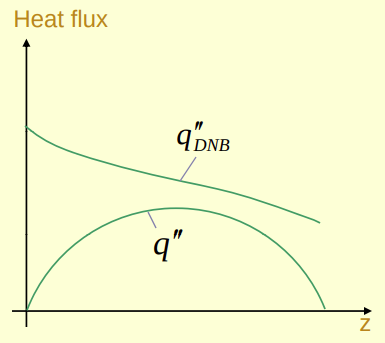
\includegraphics{simple-mdnbr-schematic.png}
\caption{Simple schematic relating local heat flux to $q^{\prime \prime}_{\text{DNB}}$.}
\label{fig:simple-mdnbr-schematic}
\end{marginfigure}
\newthought{The phenomena of} DNB depends on heat flux, local bulk temperature, pressure, and mass flux.  For a more realistic cosine-shaped flux profile we might compare the local heat flux to the heat flux that would result in DNB as illustrated in Figure \ref{fig:simple-mdnbr-schematic}. As with many of the other thermal and hydraulic phenomena covered in this course, we do not have an equation or criteria based on first principles by which to judge the onset of DNB; we require a correlation.  Thermal-hydraulic analysis codes incorporate several of these correlations; in this course I will present only one.

\section{Tong 68 DNB Correlation} \index{Tong DNB correlation}
The Tong DNB correlation is given by Equations \ref{eq:k-tong} and \ref{eq:q-tong}
\begin{marginfigure}
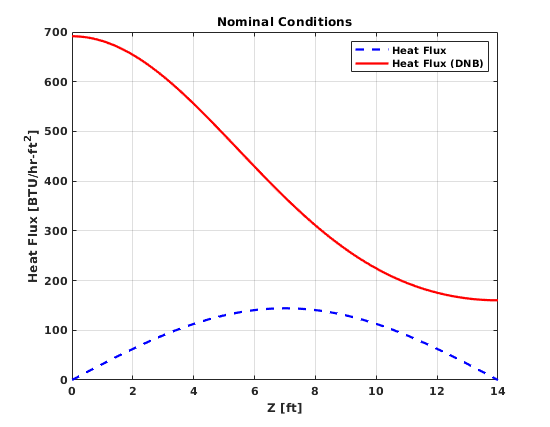
\includegraphics{tong68-dnb-nominal.png}
\caption{Calculation of DNB with Tong correlation.}
\label{fig:tong68-dnb-nominal}
\end{marginfigure}

\begin{marginfigure}
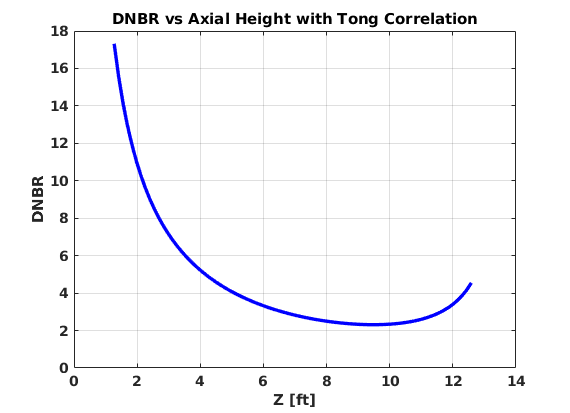
\includegraphics{mdnbr-calc-tong68.png}
\caption{Calculation of DNBR with Tong correlation.}
\label{fig:mdnbr-calc-tong68}
\end{marginfigure}

\begin{equation}
k_{\text{Tong}} = 1.76 - 7.433 x_{eq} + 12.222x_{eq}^2
\label{eq:k-tong}
\end{equation}
\begin{equation}
q^{\prime \prime}_{\text{DNB}} = k_{\text{Tong}} \frac{G^{0.4}\mu_f^{0.6}h_{fg}}{D_{e}^{0.6}}
\label{eq:q-tong}
\end{equation}
where $x_{eq}$ is equilibrium quality, $G$ is mass flux, $\mu_{f}$ is the viscosity of saturated liquid, and $h_{fg}$ is the difference in enthalpy between saturated vapor and saturated liquid at the local pressure.  For a nominal cosine-shaped flux distribution, one can calculate channel temperature, enthalpy, and equilibrium quality within the channel and, using the Tong correlation, calculate $q^{\prime \prime}_{\text{DNB}}$.  This is shown in Figure \ref{fig:tong68-dnb-nominal}. If we further compare $q^{\prime \prime}_{\text{DNB}}$ with the heat flux at that location in the channel, we can calculate the \emph{departure from nucleate boiling ratio} (DNBR).  This is shown for a portion of the channel in Figure \ref{fig:mdnbr-calc-tong68}.  If $MDNBR \le 1$, then the correlation predicts DNB will occur.  If $MDNBR > 1$ then some margin of safety exists.

\section{Variation with Plant Parameters}
\newthought{The changes of} DNB and DNBR with plant parameters may be intuitively clear to most readers.  Nonetheless it is worthwhile, I think, to do some simple calculations to observe quantitatively how variations in plant parameters affect DNB and DNBR.

\begin{marginfigure}
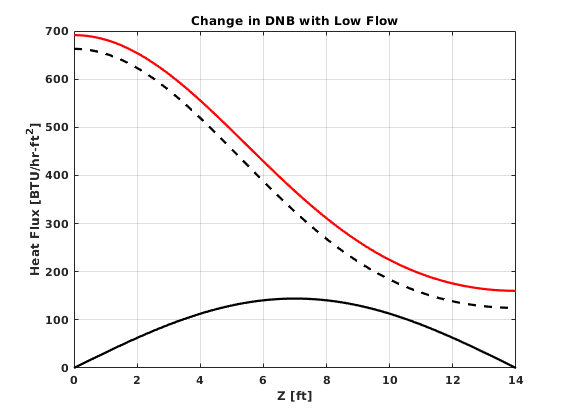
\includegraphics{tong68-dnb-reduced-flow.png}
\caption{Effect of coolant flow rate reduction on DNB.}
\label{fig:tong68-dnb-reduced-flow}
\end{marginfigure}
\begin{itemize}
\item \emph{Reduction in mass flow rate}.  Reducing mass flow rate to a channel means that the channel temperature, enthalpy, and equilibrium quality will increase more rapidly within the channel.  Onset of nucleate boiling will occur lower in the channel and $q^{\prime \prime}_{\text{DNB}}$ should be lower everywhere in the channel.  Figure \ref{fig:tong68-dnb-reduced-flow} illustrates this effect quantitatively.

\item \emph{Reduction in system pressure}.  Reducing system pressure brings the coolant closer to saturation temperature and increases equilibrium quality everywhere.  Figure \ref{fig:tong68-dnb-reduced-pressure} illustrates this.

\begin{marginfigure}
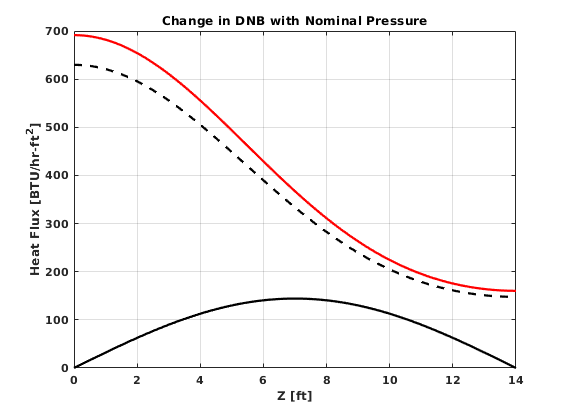
\includegraphics{tong68-dnb-reduced-pressure.png}
\caption{Effect of coolant pressure reduction on DNB.}
\label{fig:tong68-dnb-reduced-pressure}
\end{marginfigure}

\item \emph{Increase coolant inlet temperature}. Again, qualitatively this effect should be quite obvious.  Figure \ref{fig:tong68-dnb-increased-temp} shows the result quantitatively.

\begin{marginfigure}
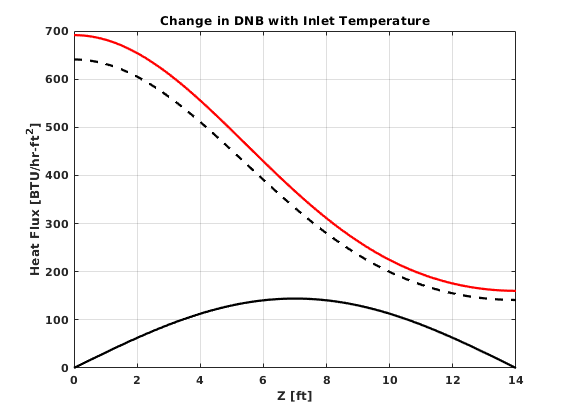
\includegraphics{tong68-dnb-increased-temp.png}
\caption{Effect of increasing coolant inlet temperature on DNB.}
\label{fig:tong68-dnb-increased-temp}
\end{marginfigure}

\item \emph{Increase power}. Core power level has a strong influence on DNB and MDNBR; increasing power, because of its effect on temperature and equilibrium quality of the coolant, reduces $q^{\prime \prime}_{\text{DNB}}$ while, since $q^{\prime \prime}$ is higher, further reduces DNBR.  These effects are illustrated in Figure \ref{fig:tong68-dnb-increased-power}.

\begin{marginfigure}
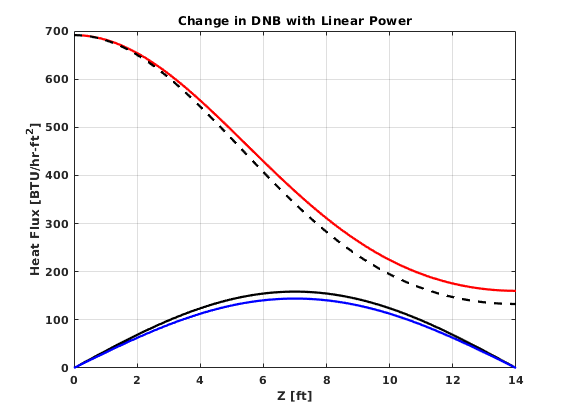
\includegraphics{tong68-dnb-increased-power.png}
\caption{Effect of increasing core power on DNB.}
\label{fig:tong68-dnb-increased-power}
\end{marginfigure}

\end{itemize}

\section{Application of Safety Factors for MDNBR}

\newthought{What may not} have yet been made explicitly clear, is that when DNB occurs, we expect fuel thermal limits to be exceeded and fuel failure to occur.  As the thermal designer of a nuclear reactor core, it is your job to prevent this.  You must ensure that DNB does not happen: not for the hottest channel in the core; despite uncertainties inherent in whatever DNB correlation you use; despite even uncertainties in plant parameters themselves; you must show that DNB does not occur during expected transients; if an accident happens, and such an accident is foreseeable, your design must make sure that DNB does not occur even under those accident conditions.  In short: you need to add margins to your design to account for a great deal of uncertainty.  

\newthought{A schematic} of how you might account for all of the above variability and uncertainty is illustrated in Figure \ref{fig:mdnbr-safety-factors}.  I conclude this lecture with a brief description of these various safety factors that should be considered.  For a more detailed discussion of this process, with application to an integral PWR, I invite you to peruse a relevant thesis.\cite{blair2003thermal}

\begin{figure}
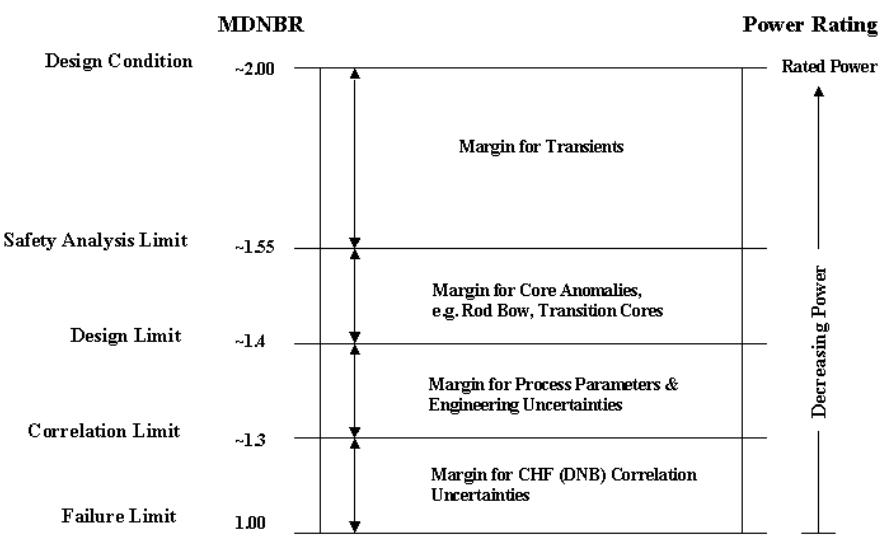
\includegraphics{mdnbr-safety-factors.png}
\caption{Safety factors to ensure DNB does not occur.} 
\label{fig:mdnbr-safety-factors}
\end{figure}

\begin{itemize}
\item \emph{Correlation limit.}  In order to provide margin to DNB, we will demand that the MDNBR be greater than 1 by some amount.  This is to account for uncertainties in the DNB correlation itself.  The correlation may have been developed with fuel assemblies of a different pitch-to-diameter ratio in mind, or the correlation may have assumed that mixing grids of a certain design were employed which, in your design, perhaps they were not, or mixing grids of less effectiveness were used instead.  For these reasons and more, margin should be provided just to account for correlation uncertainties.

\item \emph{Design limit.}  The actual reactor that gets built will be only an approximation of the reactor that exists on design drawings and is represented in computer codes.  Machine tolerances will impact actual fuel pellet diameter, cladding inside radius and thickness, reactor coolant pump volumetric flow rate, major and minor head losses: everything that you assume in your analysis can be expected to be somewhat different in practice due to manufacturing uncertainties.  Margin should be provided to account for this.

\item \emph{Safety analysis limit.}  During operations---both steady state and transient; normal operations and accident conditions---the plant will respond in ways that your analysis did not anticipate.  Within reasonable limits, additional margin should be provided to account for this.  

\item \emph{Design condition.}  Besides the variations and transients that you \emph{do not} expect, you must add margin to account for the transients you \emph{do} expect.  These margins can be quite large and rely extensively on detailed system analysis codes to allow you to estimate the impact of design-basis transients such as loss of cooling, loss of flow, uncontrolled rod withdrawal among many others.  
\end{itemize}

In the end, the thermal-hydraulic designer will determine the power level, assumed power profile, and core geometry such that the core will be ``safe'' while accounting for all of the aforementioned uncertainties.  If the \emph{reactor physicist} ensures the reactor will go critical and produces the required amount of power for the desired length of time, the \emph{reactor engineer} or \emph{thermal-hydraulicist} will ensure ensure the core can be safely cooled and all materials will remain within their thermal limits under all conditions.
  
